\documentclass[a4paper]{article}
\usepackage[letterpaper, margin=1in]{geometry} % page format
\usepackage{listings} % this package is for including code
\usepackage{graphicx} % this package is for including figures
\usepackage{amsmath}  % this package is for math and matrices
\usepackage{amsfonts} % this package is for math fonts
\usepackage{tikz} % for drawings
\usepackage{hyperref} % for urls

\title{Homework 02}
\author{Brian Henderson}
\date{10/16/17}

\begin{document}
\lstset{language=Python}

\maketitle

\section{Overview}
Run experiments using RNNs on the lab "Applying RNNs/LSTMs to MNIST." Vary the number of hidden units (neurons) exponentially as follows, 16, 32, 64, 128, 256, 512, 1024, 2048, and 4096; also vary the learning rate exponentially as follows: 0.00001, 0.0001, 0.001, 0.01, 0.1, and 1.0. Discuss the results and interpret them; what is this telling you about the training of an LSTM with respect to the number of neurons or learning rate or both? What can you learn from this?
\\
\section{Results}
\begin{center}
\begin{tabular}{l*{8}{c}r}
Neurons/Learning Rate        & 0.00001 & 0.0001 & 0.001 & 0.01 & 0.1  & 1.0 \\
\hline
16	& 0.1232 & 0.3784 & 0.8593 & 0.9413 & 0.8370 & 0.1032 \\
32	& 0.1250 & 0.6993 & 0.9246 & 0.9669 & 0.7862 & 0.1010 \\
64	& 0.2697 & 0.8163 & 0.9538 & 0.9694 & 0.8924 & 0.1009 \\
128	& 0.5023 & 0.9050 & 0.9684 & 0.9792 & 0.1032 & 0.1028 \\
256	& 0.6402 & 0.9163 & 0.9710 & 0.9719 & 0.6887 & 0.0958 \\
512	& 0.7805 & 0.9395 & 0.9624 & 0.1135 & 0.1032 & 0.0958 \\
1024	& 0.8285 & 0.9465 & 0.9645 & 0.3337 & 0.0979 & 0.0974 \\
2048	& 0.0865 & 0.9497 & 0.9694 & 0.1009 & 0.1001 & 0.0958 \\
4096	& 0.9443 & 0.9596 & 0.9402 & 0.1032 & 0.1290 & 0.0909 \\

\end{tabular}
\end{center}

\section{Analysis}
After running the 56 different experiments with the various learning rates and neurons, many interpretations came about. As the hidden layers (neurons) increased, so did the time to complete the optimization. The learning rate had an impact on the final testing accuracy in respect to the number of neurons. However, the experiment results show that no matter how many neurons there were, some of the learning rates had relatively consistent testing accuracy results, with no outstanding outliers. The learning rate of 0.001 had very consistent results, with all testing accuracy’s within the range of 0.85 0- 0.975. The experiments with more neurons had better test accuracy’s with the lower learning rates compared to the higher learning rates The experiment with the highest testing accuracy was using a model with 128 neurons and a learning rate of 0.01. From the results of this set of experiments, it can be learned that in order to get a quality test accuracy, it is not necessary to have a high amount of hidden layers/neurons, as the learning rate is the true factor is getting quality test accuracy’s.

\begin{figure}
   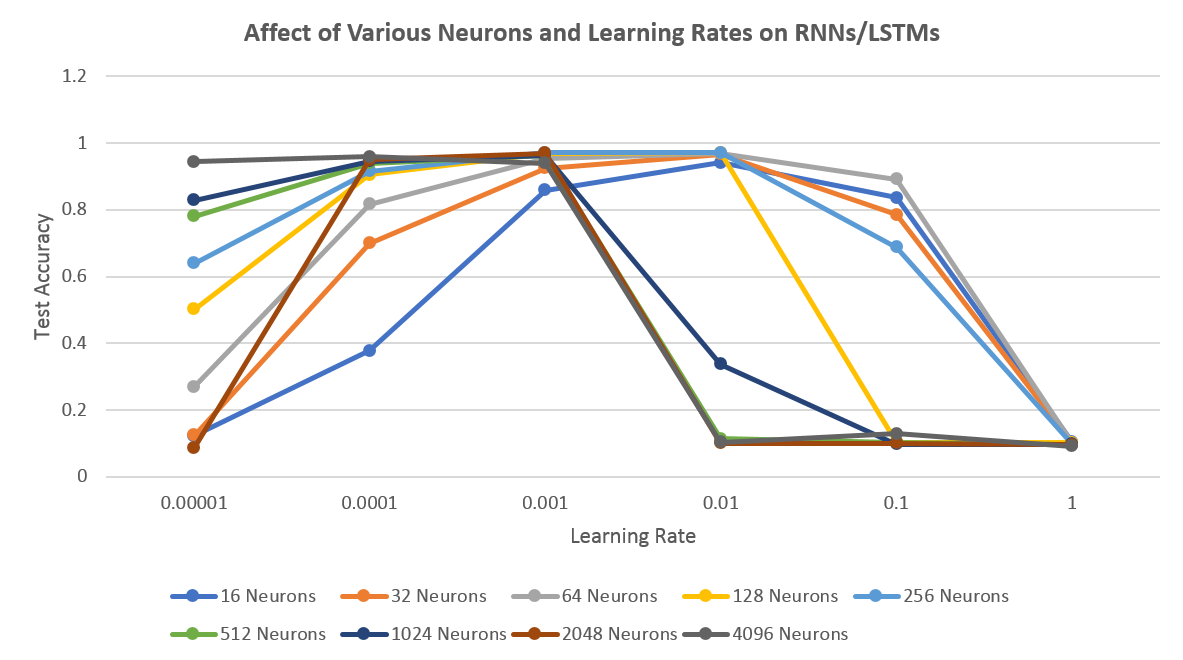
\includegraphics[width=\linewidth]{resultsGraph.png}
   \caption{ Experiment Results Visualization}
   \label{fig:results}
\end{figure}

\end{document}